\section{Scheduling}
Un sistema operativo deve allocare risorse tra i processi, tra le risorse quella piú ovvia é il processore, l' uso del
    processore é detto scheduling, la metodologia che gestisce l'uso del processore é detta politica di scheduling,
    lo scopo dello scheduling é assegnare ad ogni processore qualcosa de eseguire, bisogna quindi che lo scheduling
    sia il piú efficiente possibile, tenendo conto di vari aspetti:
    \begin{itemize}
        \item tempo di risposta (Tendo a minimizzare)
        \item throughput (Tendo a massimizzare)
        \item efficienza del processore (Tendo a massimizzare)
    \end{itemize}
    altri obbiettivi dello scheduling é non fare favoritismi tra i processi, tuttavia nei moderni sistemi operativi
    esiste la priorità dei processi, quindi alcuni processi vengono privilegiati rispetto altri, inoltre lo scheduling
    deve evitare lo starvation, ovvero che un processo non venga mai eseguito, noon lasciare mai il processore inattivo,
    avere un overhead basso (il tempo per fare lo scheduling deve essere il piú basso possibile),
    \subsection{Tipi di scheduling}
    \begin{itemize}
        \item Long-term scheduling: decide quali processi devono essere caricati in memoria
        \item Medium-term scheduling: decide quali processi devono essere spostati dalla memoria principale alla memoria secondaria
        \item Short-term scheduling: decide quale processo deve essere eseguito sulla CPU
        \item I/O scheduling: decide quale processo deve essere eseguito sul dispositivo di I/O
    \end{itemize}
    \begin{figure}[H]
        \centering
        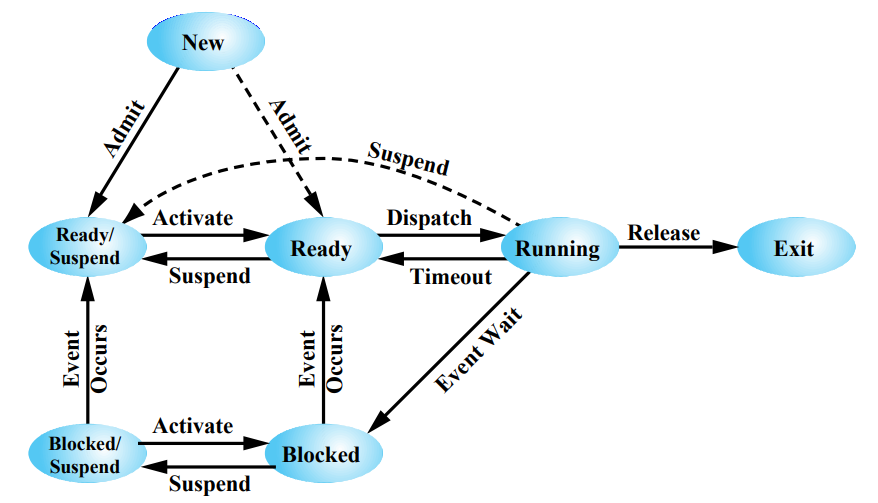
\includegraphics[width=0.5\textwidth]{immagini/7State}
        \caption{Tipi di scheduling}
    \end{figure}
    abbiamo visto che si di ready che di blocked ci sono le versioni suspended (sono in memoria secondaria), molte
    delle transizioni sono dovute allo scheduler, quello che decide se un processo appena creato Ready o Ready Suspended
    é il long-term scheduler, il medium-term decide tra le versioni suspended e non suspended, il short-term scheduler
    decide se un processo é Ready o Running, il I/O scheduler decide se un processo é Blocked o Ready
    \begin{figure}[H]
        \centering
        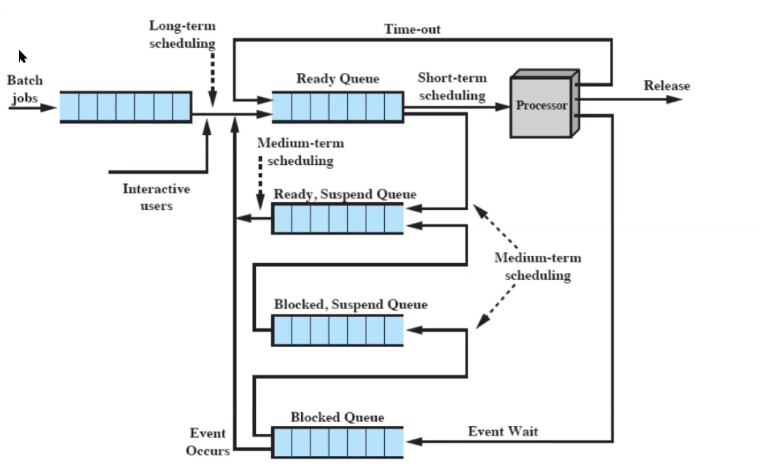
\includegraphics[width=0.5\textwidth]{immagini/implementazioneScheduling}
        \caption{Tipi di scheduling}
    \end{figure}
    lo scheduling fa una distinzione tra processi interattivi e processi batch, i processi in batch hanno una coda, mentre
    quelli interattivi cercano direttaqmente di essere eseguiti, Il long-term come detto sopra decide se i processi sono
    messi in ready o ready suspended, il medium term scheduler decide se un processo é messo in ready o ready suspended
    oppure blocked o blocked suspended e viceversa, il short term scheduler decide se un processo é messo in running o blocked
    \subsection{Long-term scheduling}
    Decidide quali programmi sono ammessi nel sistema, spesso segue una logica FIFO (First In First Out),
    spesso é un FIFO "Corretto, tenendo conto di criteri come la priorità, il tempo di esecuzione, ecc.

    Inoltre controlla il grado di multiprogrammazione, ovvero il numero di processi che possono essere eseguiti
    contemporaneamente, il grado di multiprogrammazione é il numero di processi che possono essere eseguiti
    contemporaneamente,

    Piú processi ci sono, piú é piccola la percentuale di tempo per cui ogni processo viene eseguito.

    Le strategie di scheduling sono:
    \begin{itemize}
        \item i lavori batch vengono accodati e il LTS li prende man mano che il processore é libero
        \item I lavori interattivi vengono ammessi fino a saturazione del sistema
        \item Se si sa quali processi sono I/O bound e quali sono CPU bound, si possono fare scelte migliori facendo un giusto mix tra due tipi
        \item Se si sa quali processi fanno richieste a quali dispositivi, di I/O, fare in modo di bilanciare le richieste
    \end{itemize}
    Il Long-term scheduler puó essere chiamato anche quando non ci sono nuovi processi, ad esempio quando termina un processo oppure
    quando un processo é idle da troppo tempo.

    \subsection{Medium-term scheduling}
    Il medium-term scheduler decide se bisogna fare degli aggiustamenti tra RAM e Disco, il motivo principale é quello di gestire
    la multiprogrammazzione, se terminano 10 processi ad esempio, il medium term scheduler decide quali processi ready
    presenti in memoria secondaria devono essere spostati in memoria principale, il medium term scheduler é chiamato anche
    \subsection{short-term scheduling}
    Il short-term scheduler é chiamato anche dispatcher, decide quale processo deve essere eseguito sulla CPU,
    ed é quello eseguito piú frequentemente.viene invocato in seguito a:
    \begin{itemize}
        \item interruzzioni di clock
        \item interruzzioni di I/O
        \item chiama di sistema
        \item segnali
    \end{itemize}

    Lo scopo dello short-term scheduler é quello di allocare tempo di esucozione tra i processori, per ottimizzare
    il comportamento dell'intero sistema, per valutare quindi una politica di scheduling bisogna valutare:
    \begin{itemize}
        \item Utente: tempo di risposta, tempo di esecuzione
        \item Sistema: throughput, efficienza del processore
    \end{itemize}
    L' altra categoria é quella se sono criteri se sono criteri prestazionali (quantitativi) oppure quelli non
    prestazionali (qualitativi) che sono piú difficili da misurare.
    \subsubsection{Criteri Utente}
    Prestazionali :
        \begin{itemize}
        \item   \textbf{Turnaround time}: tempo tra la creazione e la terminazione di un processo
        \item  \textbf{Tempo di risposta}: tempo tra la creazione e la prima risposta
        \item  \textbf{Deadline}: tempo entro il quale un processo deve essere completato
    \end{itemize}
    Non Prestazionali:
    \begin{itemize}
        \item \textbf{Predictability}: quanto é prevedibile il tempo di esecuzione
    \end{itemize}
    \subsubsection{Criteri di sistema}
    Prestazionali:
    \begin{itemize}
        \item \textbf{Throughput}: numero di processi completati in un certo intervallo di tempo
        \item \textbf{Efficienza del processore}: percentuale di tempo in cui il processore é utilizzato
    \end{itemize}
    Non Prestazionali:
    \begin{itemize}
        \item \textbf{Equità}: tutti i processi devono avere la stessa possibilitá di essere eseguiti
        \item \textbf{Enforces priorities}: i processi con priorità piú alta devono essere eseguiti prima
        \item \textbf{Balancing resources}: bilanciare l'uso delle risorse
        \end{itemize}
    \subsection{Turnaround time}
    Il turnaround time é il tempo tra la creazione e la terminazione di un processo, comprende i vari tempi di attesa (I/O, CPU, ecc.)
    si usa spesso per processi non interattivi.
    \subsection{Tempo di risposta}
    Il tempo di risposta é il tempo tra la creazione e la prima risposta, é importante per i processi interattivi (es. un utente che clicca su un bottone)
    lo scheduler in questo caso ha un duplice obbiettivo per lo scheduler: minimizzare il tempo di risposta medio
    e massimizzare il numero di utenti che hanno un risposta veloce.
    \subsection{Deadline}
    La deadline é il tempo entro il quale un processo deve essere completato, é importante per i processi real-time,
    un buon dispatcher deve massimizzare il numero di scadenze rispettate, per quanto riguarda invece la Predictability
    se lancio tante volte lo stesso processo, il tempo di esecuzione deve essere sempre lo stesso, altrimenti il
    dispatcher non é prevedibile.
    \subsection{Throughput}
    Il throughput é il numero di processi completati in un certo intervallo di tempo, ovviamente l' obbietti é massimizzare
    il throughput, é una misura di quanto lavoro viene effettuato.
    \subsection{Utilizzo del processore}
    L' utilizzo del processore é la percentuale di tempo in cui il processore é utilizzato, ovviamente l' obbiettivo é massimizzare
    l' utilizzo del processore, quindi il processore non deve mai essere inattivo, questo é un criterio molto costosi condivisi
    tra piú utenti.
    \subsection{Bilanciamento delle risorse}
    Lo scheduler deve bilanciare l'uso delle risorse, ad esempio se un processo é CPU bound, non ha senso assegnargli un
    tempo di I/O, quindi lo scheduler deve bilanciare l'uso delle risorse, quindi processi che utilizzano meno le risorse attualmente
    piú usate devono essere favoriti.
    \subsection{Fairness e Priorità}
    La fairness é il concetto che tutti i processi devono avere la stessa possibilitá di essere eseguiti, per cui non sono
    presenti favoritismi, a meno che non ci siano priorità, in questo caso i processi con priorità piú alta devono essere eseguiti
    prima, inoltre questo causera la creazioni di code di processi, quindi lo scheduler deve essere in grado di gestire le code
    di processi.
    \subsection{Prioritá e Starvation}
    La prioritá ha un problema, ovvero che puó indurre starvation, esempio: se un processo ha una bassa priorità, potrebbe
    non essere mai eseguito, quindi lo scheduler deve evitare lo starvation, ovvero che un processo non venga mai eseguito,
    per evitare lo starvation si puó usare la politica di aging, ovvero aumentare la priorità di un processo che non viene mai eseguito.
    \subsection{Politiche di scheduling}
    \begin{figure}[H]
        \centering
        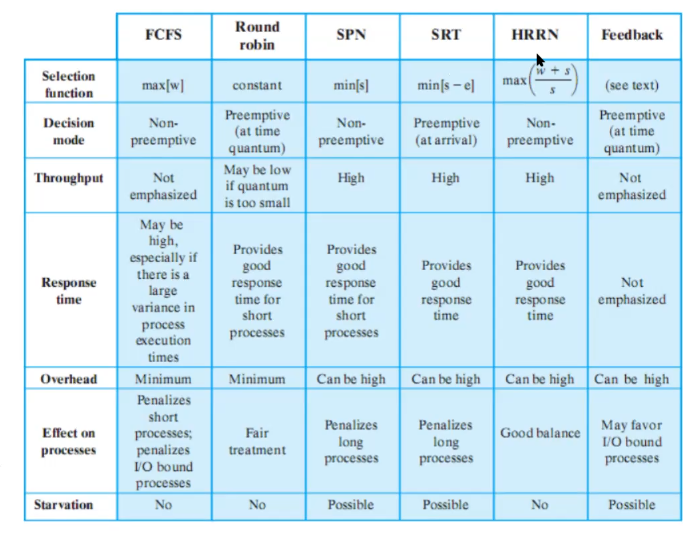
\includegraphics[width=1\textwidth]{immagini/PoliticheDiScheduling}
        \caption{Politiche di scheduling}
    \end{figure}
    Raramente si usa una sola politica di scheduling, si usano piú politiche di scheduling, inoltre non si
    utilizzano gli algoritmi di scheduling implementate, ma revisioni di esse.
    \subsection{Selection Function}
    La selection function é quella che sceglie effetivamente quale processo deve essere eseguito,
    la scelta viene fatta in base a vari criteri:
    \begin{itemize}
        \item w = tempo di attesa
        \item e = tempo trascorso in esecuzione
        \item s = tempo totale richiesto (stimato), incluso quello giá servito (e)
    \end{itemize}
    \subsection{Decision Mode}
    Specifica in quali istanti di tempo la funzione di selezione viene invocata, ci sono 2 possibili modi:
    \begin{itemize}
        \item Non pre-emptive: la funzione di selezione viene invocata solo quando il processo in esecuzione termina
        \item Pre-emptive: la funzione di selezione viene invocata ad intervalli regolari
    \end{itemize}
    \subsubsection{Pre-emptive - Non pre-emptive}
    Non pre-emptive: se un processo é in esecuzione, allora arriva o fino a terminazione of fino ad un I/O, non gli tolgo il processore

    Pre-emptive: Il sistema operativo puó interrompere un processo in esecuzione per eseguire un altro processo, in questo caso il processo
    passera da running a ready, la preemption di un processo puó avvenire o pre l'arrivo di nuovi processi (appena creati) o per un interrupt di I/O,
    oppure per interrupt di clock, quest'ultimo é periodico per evitare che alcuni processi monopolizzino il processore.
    \subsection{ESEMPIO}
    Scenario Comune :
    \begin{table}[H]
        \raggedright
        \begin{tabular}{|c|c|c|}
            \hline
            \textbf{Processo} & \textbf{Tempo di arrivo} & \textbf{Tempo di esecuzione} \\
            \hline
            A & 0 & 3   \\
            \hline
            B & 2 & 6 \\
            \hline
            C & 4 & 4  \\
            \hline
            D & 6 & 5  \\
            \hline
            E & 8 & 2  \\
            \hline
        \end{tabular}
    \end{table}
    \subsection{First Come First Served}
    Tutti i processi sono aggiunti alla coda ready, é non pre-emptive, quando il processo ha finito di essere eseguito, si passa
    al processo che ha aspettato di piú nella coda.
    \begin{figure}[H]
        \centering
        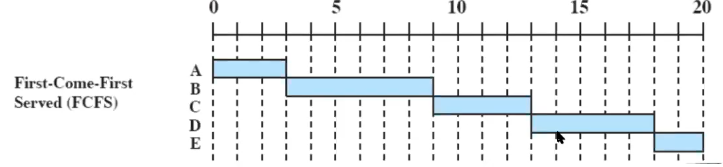
\includegraphics[width=0.75\textwidth]{immagini/FCFS}
        \caption{First Come First Served}
    \end{figure}
    L' algoritmo é molto semplice, é anche molto equo, dal punto di vista del sistema operativo, un processo corto
    deve aspettare che altri processi terminino, favorisce i processi CPU bound, per cui degenera perché un processo 
    monopolizza il processore.
    \subsection{Round Robin}
        \begin{table}[H]
        \raggedright
        \begin{tabular}{|c|c|c|}
            \hline
            \textbf{Processo} & \textbf{Tempo di arrivo} & \textbf{Tempo di esecuzione} \\
            \hline
            A & 0 & 3   \\
            \hline
            B & 2 & 6 \\
            \hline
            C & 4 & 4  \\
            \hline
            D & 6 & 5  \\
            \hline
            E & 8 & 2  \\
            \hline
        \end{tabular}
    \end{table}
    Il round robin usa la preemption, basandosi su un clock, Talvolta chiamato time slicing, perché ogni processo
    ha una fetta di tempo, é un algoritmo di scheduling per processi interattivi.
    \begin{figure}[H]
        \centering
        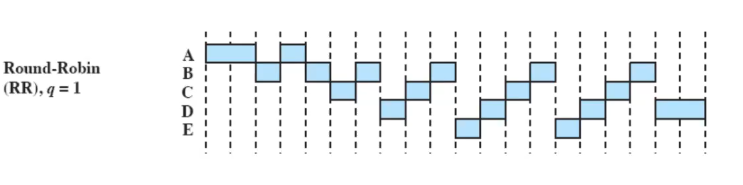
\includegraphics[width=0.75\textwidth]{immagini/RoundRobin}
        \caption{Round Robin}
    \end{figure}
    in questo caso il processo E finisce prima rispetto all'algoritmo FCFS, nel
    caso ci sia una coda si utilizza una politica FIFO, quando un processo finisce il tempo di esecuzione viene ri-aggiunto alla coda


    \textbf{Quanto di tempo} é un intervallo di tempo che viene assegnato ad ogni processo e rappresenta il tempo per il quale il processo ha accesso
    al processore,il quanto di tempo deve essere non troppo piú grande del tipico tempo di interazione di un processo.
    \begin{figure}[H]
        \centering
        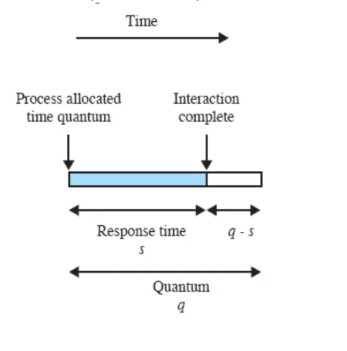
\includegraphics[width=0.75\textwidth]{immagini/Quanto di tempo Giusto}
        \caption{Quanto di tempo piú grande del tempo di interazione}
    \end{figure}
    Se invece uno sceglie il quanto di tempo piú piccolo, il processo che va in esecuzione avrebbe bisogno di piú tempo del quanto,
    prima della risposta gli viene tolto il processore, questo significa che il tempo di risposta é piú lungo.
    \begin{figure}[H]
        \centering
        \includegraphics[width=0.75\textwidth]{immagini/Quanto piú piccolo}
        \caption{Quanto di tempo piú piccolo del tempo di interazione}
    \end{figure}
    Nel momento in cui si sceglie di usare il round robin, si fa una analisi statistica di quantitá di tempo di esecuzione
    necessaria per i processi per assegnare il quanto di tempo, invece se assegno un quanto di tempo troppo grande, allora
    il round robin diventa un FCFS.
    \subsubsection*{CPU bound vs I/O bound}
    C'é un problema con il round robin, per quello che riguarda i processi CPU bound contro i processi I/O bound,
    anche con il round robin anche i processi CPU bound vengono favoriti, perché i processi CPU bound utilizzano
    tutto il quanto di tempo, mentre i processi I/O bound non utilizzano tutto il quanto di tempo in caso di richiesta
    bloccante, dal punto di vista dell'equitá non va bene, é stata proposta una soluzione \textbf{Round Robin Virtuale}
    che funziona come il round robin, ma se un processo fa una richiesta bloccante, allora il processo non va in una coda
    dei ready dopo aver completato la richiesta di I/O come succede normalmente, invece con il round robin virtuale
    esiste una coda ausiliaria, che accoda i processi che sono stati blocked, dopo di che il dispatcher sceglie prima
    la coda ausiliaria e poi la coda dei ready.
    \begin{figure}
        \centering
        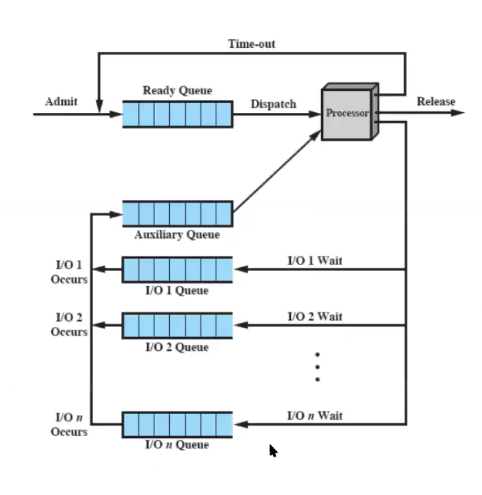
\includegraphics[width=0.75\textwidth]{immagini/RoundRobinVirtuale}
        \caption{Round Robin Virtuale}
    \end{figure}
    Da notare che scegliendo dalla coda ausiliaria, rimando i processi in esecuzione solo per il quanto di tempo che gli rimaneva

    \subsection{Shortest Process Next}
    Il Shortest Process Next é un algoritmo non pre-emptive, per implentarlo é necessario sapere quanto tempo di escuzione il
    processo richiede, la logica per scegliere il prossimo processo é quello col tempo di esecuzione piú breve,
    questo fa si che i processi corti scavalchino i processi piú lunghi.
    \begin{figure}[H]
        \centering
        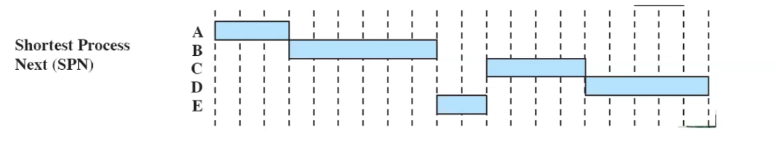
\includegraphics[width=0.75\textwidth]{immagini/SPN}
        \caption{Shortest Process Next}
    \end{figure}
    Il problema é quello di dover dare una stima del tempo di esecuzione dei processi,
    ma anche assumendo di avere una buona stima, dal punto di vista dei criteri utente, la predictability di processi
    lunghi é ridotta, questo addirittura potrebbe creare starvation, perché i processi corti vengono sempre eseguiti
    mentre i processi lunghi potrebbero rimanere in attesa per sempre, se il tempo stimato é sbagliato il sistema operativo
    potrebbe abortire il processo.
    \subsubsection*{Stimare il tempo di esecuzione}
    Per stimare il tempo di esecuzione, ci sono alcuni processi che vengono eseguiti piú volte,
    quindi per questo tipo di processi si puó guardare il passato per prevedere il futuro, ad esempio facendo una
    media dei tempi di esecuzione passati,
    \begin{equation}
    S_n_+_1 = \frac{1}{n} \sum_{i=1}^{n} T_i\label{eq:Media dei tempi di esecuzione}
    \end{equation}
    per fare questo significa che il dispatcher deve tenere traccia del tempo di esecuzione di ogni processo, questo
    potrebbe richiedere molta memoria, l'altro modo é quello di ricordarmi solo l'ultimo tempo di esecuzione e l'ultima
    stime con :
    \begin{equation}
        S_n_+_1 = \frac{1}{n}T_n + \frac{n-1}{n}S_n\label{eq:Mi ricordo solo l'ultimo tempo di esecuzione e l'ultima stima}
    \end{equation}
    questa si puo' generalizzare con un parametro $\alpha$, dove $\alpha$ é un valore tra 0 e 1 otteniamo:
    \begin{equation}
        S_n_+_1 = \alpha T_n + (1-\alpha)S_n\label{eq:formula con $\alpha$}
    \end{equation}
    formula media esponenziale:
    \begin{equation}
        S_n_+_1 = \alpha T_n + ... + (1-\alpha)^iT_n_-_i +...+ (1-\alpha)^nS_1\label{eq: Exponential Averaging }
    \end{equation}
    \begin{figure}
        \centering
        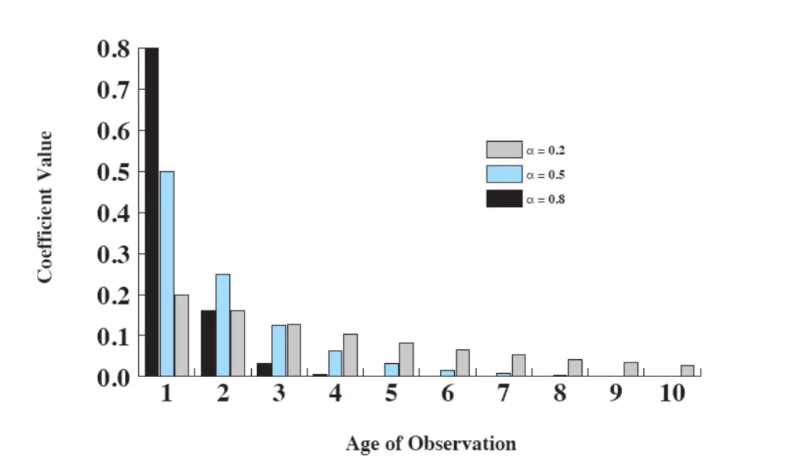
\includegraphics[width=0.75\textwidth]{immagini/AnalisiDiAlphaSpn}
        \caption{Analisi di Alpha}
    \end{figure}
    Piú $\alpha$ é vicino a 1, piú sparisce velocemente il passato, questo serve a capire che con un buon $\alpha$ si 
    possono fare delle ottime previsioni.
    \subsubsection*{Esempio}
    \begin{figure}[H]
        \centering
        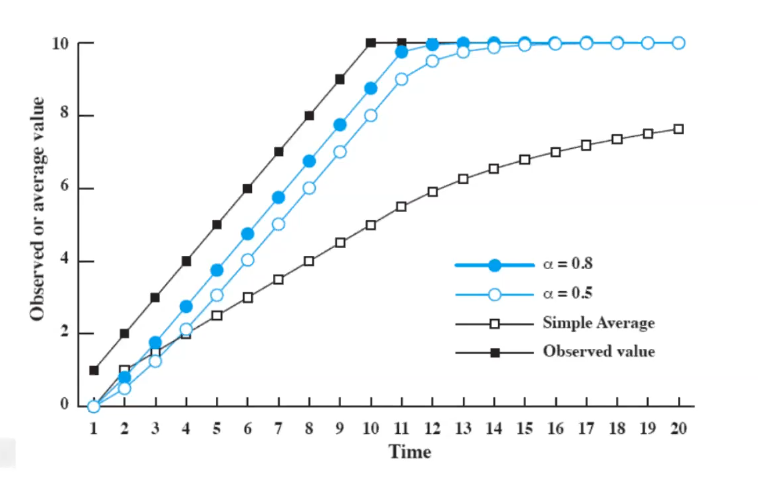
\includegraphics[width=0.75\textwidth]{immagini/EsempioExponentialAveraging}
        \caption{Esempio 1}
    \end{figure}
    Abbiamo fissato un processo e diciamo che la sua prima istanza cresce e poi si stabilizza, se io facessi
    semplicemente la media, quello che la media predirebbe sarebbe un valore lontano dall'obbiettivo, invece
    se uso degli $\alpha$ fissi, siamo molto piú vicini alla curva reale.
    \begin{figure}[H]
        \centering
        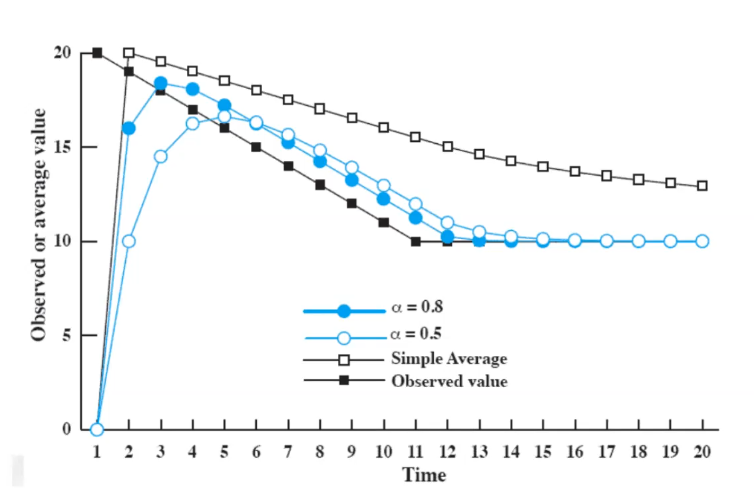
\includegraphics[width=0.75\textwidth]{immagini/EsempioExponentialAveraging2}
        \caption{Esempio 2}
    \end{figure}
    Praticamente dopo un certo tempo, i valori vecchi vengono dimenticati, specialmente per $\alpha$ grandi
    \subsection{Shortest Remaining Time}
    Lo Shortest Remaining Time é una versione pre-emptive dello Shortest Process Next, é preemptive sulla base che arrivi
    un nuovo processo, quindi io stimo il tempo rimanente per l'esecuzione, se il tempo rimanente di un processo in coda é minore
    del tempo di esecuzione del processo in esecuzione, allora il processo in esecuzione viene pre-empted.
    \begin{figure}[H]
        \centering
        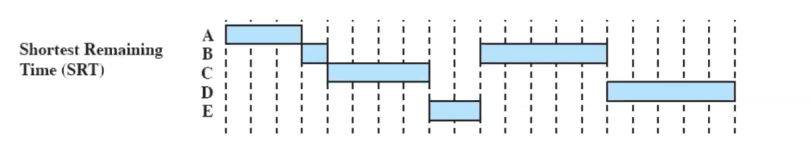
\includegraphics[width=0.75\textwidth]{immagini/SRT}
        \caption{Shortest Remaining Time}
    \end{figure}
    I processi lunghi comunque possono soffrire di starvation, perché i processi corti vengono sempre eseguiti, anche in
    questo caso é necessario sapere il tempo di esecuzione.
    \subsection{Highest Response Ratio Next}
    L' algoritmo Highest Response Ratio Next é un algoritmo non pre-emptive, é una versione migliorata dello Shortest Process Next,
    che risolve il problema dello starvation, é basato sul tempo di attesa, il tempo di esecuzione e il tempo totale richiesto,
    é un compromesso tra quanto tempo sto aspettando e quanto tempo ci metto ad eseguire.

    L'algoritmo massimizza il seguente rapporto:
    \begin{equation}
        \frac{w+s}{s} = \frac{tempo trascorso in attesa + tempo totale richiesto}{tempo totale richiesto}
    \end{equation}
    \begin{figure}[H]
        \centering
        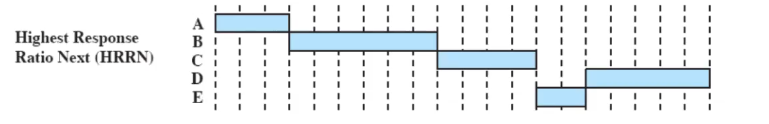
\includegraphics[width=0.75\textwidth]{immagini/HRRN}
        \caption{Highest Response Ratio Next}
    \end{figure}
    \subsectioni*{Diagramma Riassuntivo}
    \begin{figure}[H]
        \centering
        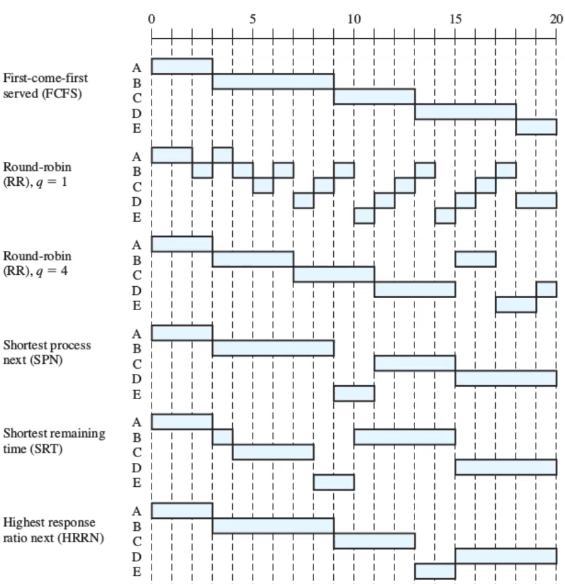
\includegraphics[width=0.75\textwidth]{immagini/RiassuntoScheduling}
        \caption{Diagramma Riassuntivo}
    \end{figure}
    \subsection{Scheduling in Unix}
    Unix combina prioritá e ruond robin, un processo quindi resta in esecuzione per al massimo un secondo, a meno che non termini
    o si blocchi, esistono diverse code a seconda della prioritá; all'interno di ciascuna coda viene eseguito il round robin.
    Le prioritá vengono ricalcolate ogni secondo, piú un processo resta in esecuzione, minore sará la sua prioritá quando
    viene rimesso in coda(feedback). Le prioritá iniziali vengono assegnate in base al tipo di processo :
    \begin{itemize}
        \item swaper (alta)
        \item controllo di un dispositivo di I/O a blocchi
        \item gestione di file
        \item controllo di un dispositivo di I/O a caratteri
        \item processi utente (basso)
    \end{itemize}
    la formula per lo scheduling é
    \begin{equation}[H]
        CPU_j(i)= \frac{CPU_J(i-1)}{2}
    \end{equation}
    che viene poi utilizzata nella formula per il calcolo della prioritá
    \begin{equation}[H]
        P_j(i) = Base_Priority_j + CPU_j(i) + Nice_j
    \end{equation}
    \begin{itemize}
        \item \textbf{J} é un indice che indica i processi \textbf{ready}
        \item \textbf{Base\_Priority\_j} é la prioritá iniziale del processo (da 0 a 4)
        \item \textbf{Nice\_j} Ricordano che il valore della prioritá piú é alto piú la prioritá é bassa, l'idea
        dietro di nice_j é la capacitá di un processo di auto-declassarsi, é usata  nei processi di sistema.
        \item \textbf{CPU\_j(i)} É una misuta di quanto il processo j ha usato il processore nell'intervalli i, con
        exponential averaging dei tempi passati, in particolare con \alpha = \frac{1}{2}
    \end{itemize}
    \subsubsection*{Esempio}
    \begin{figure}
        \centering
        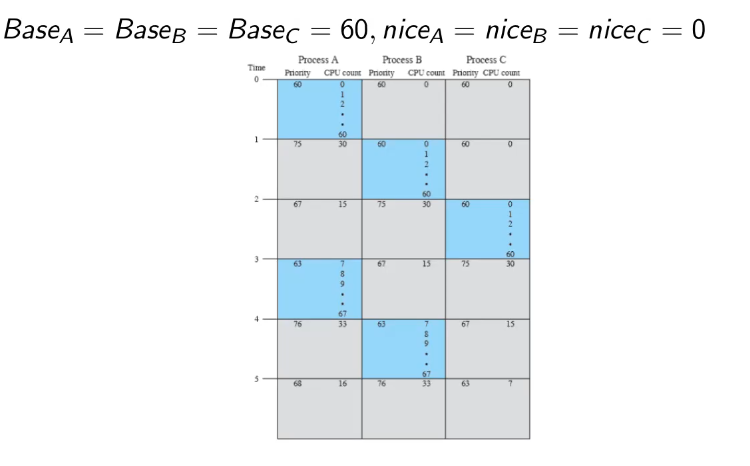
\includegraphics[width=0.75\textwidth]{immagini/EsempioSchedulingUnix}
        \caption{Esempio Scheduling Unix}
    \end{figure}
    Supponiamo che ci siano 3 processi, A, B e C, con il nice = 0 e la base priority = 60, e che il processo A sia in esecuzione
    quindi si comincia da 60 e poi bisogna aggiungere CPU_j che inizialmente é 0, chi non é in esecuzione (B e C) non lo incrementana,
    se il processo A é in esecuzione per un secondo, allora CPU_j = 30 (applicare la formula), finito il tempo di esecuzione,
    si calcola la nuova prioritá (P_j) e si rimette in coda, dopo di che lo scheduler controlla il processo con la prioritá piú alta,
    dopo un secondo quando vengono ricalcolate le prioritá, la prioritá di A diventa 67 perché:
    \begin{equation}
        CPU_j(60) = \frac{60}{2} = 15
    \end{equation}
    \begin{equation}
        P_j = 60 + \frac{CPU_j}{2} + 0 = 75
    \end{equation}
    questa operazione viene fatta per tutti i processi ogni secondo.
    Il Round robin é virtuale, quindi se un processo é bloccato, non viene messo in coda, ma viene messo in una coda ausiliaria,
    e viene eseguito prima di quelli in coda quando torna disponibile.
    \subsection{Architetture Multicore}
    Ci sono diversi modi per avere piú modi per avere piú core:
    \begin{itemize}
        \item \textbf{Cluster} : ogni processore ha la propria RAM
        \item \textbf{Processori specializzati}: un processore per le operazioni di I/O, un processore per le operazioni di calcolo
        \item \textbf{Multi-processore}: Condividono la stessa RAM,un solo sistema operativo controlla tutto
    \end{itemize}
    Noi ci concentreremo sui multi-processori, nel caso di un sistema mono-processore, ho n processi e decido quale di
    essi va in esecuzione, nel caso di un sistema multi-processore, ho n processi e m processori, quindi devo decidere
    se devo fare un Assegnaemnto Statico o Dinamico.
    \subsubsection*{Assegnamento Statico}
    Con l' assegnamento statico, ad ogni processo viene assegnato un processore, per tutta la sua durata andrá in esecuzione su quel
    processore, si puó anche usare uno scheduler per ogni processore, i vantaggi sono che é facile da implementare, ma il problema
    é che un processore potrebbe rimanere idle.
    \subsubsection*{Assegnamento Dinamico}
    Per migliorare lo svantaggio dello statico, un processo, nel corso della sua vita, potrá essere eseguito su diversi processori
    , il sistema operativo potrebbe essere sempre eseguito su un processore fisso, questa cosa é semplice da realizzare mentre solo i processi
    utenti possono essere assegnati a processori diversi, un altra scelta é quella di eseguire il sistema operativo su tutti i processori
    ma questo causa piú overhead.
    \subsection{Scheduling in Linux}
    Linux cerca la velocitá di esecuzione, tramite semplicitá, per questo non esiste long-term e medium-term scheduler (non
    ha senso perché non esistono processi suspended), Un embrione del long-term c'é perché quando creo un processo il sistema
    potrebbe essere giá saturo.
    \subsubsection*{Come Funziona}
    Ci sono le runqueue(Code dei Ready), e le wait queues (code dei blocked), Le wait queues sono condivise tra i processori,
    mentre le runqueue sono separate, ogni processore ha la sua runqueue. Essenzialmente lo scheduling é derivato da quello
    di UNIX, quindi é pre-emptive, a prioritá dinamica, ma con importanti correzzioni :
    \begin{enumerate}
        \item essere veloce, ed operare quasi in O(1)
        \item servire in modo appropriato i processi real-time
    \end{enumerate}
    Linux istruisce l'hardware di mandare un timer interrupt ogni 1ms:
    \begin{itemize}
        \item piú lungo abbiamo problemi per appicazioini real-time
        \item piú corto arrivano troppi interrupt, per cui abbiamo tanto tempo speso in Kernel Mode e quindi meno tempo
        per i processi utenti
    \end{itemize}
    percui il quanto di tempo per ciascun processo é un multiplo di 1ms.\\


    Linux considera tre tipi di processi:
    \begin{itemize}
        \item \textbf{Real-time} : hanno prioritá fisse, e vengono eseguiti prima di tutti gli altri
        \item \textbf{Interattivi} : hanno prioritá dinamiche, e vengono eseguiti dopo i real-time
        \item \textbf{Batch} : hanno prioritá dinamiche, e vengono eseguiti dopo gli interattivi
        \end{itemize}
    \subsubsection*{Interattivi}
    Non appena si agisce sul mouse o sulla tastier, é importante dare lor la CPU in 150ms al massimo
    \subsubsection*{Batch}
    Lo scheduler puó decidere di penalizzare i processi batch, perché non sono interattivi, quindi non c'é bisogno di dare
    un feedback immediato all'utente.
    \subsubsection*{Real-time}
    Gli unici riconosciuti come tali da Linux: Il loro codice sorgente usa la system call \textbf{sched\_setscheduler}
    ,per gli altri usa un'euristica, esempi di sistemi real-time sono riproduttori di audio e video, controllori, ... ma normalmente
    sono usati dai KLT.
    \subsubsection*{Classi di scheduling}
    Linux ha 3 classi di scheduling:
    \begin{itemize}
        \item \textbf{SCHED\_FIFO e SCHED\_RR } : fanno riferimento ai processi real-time
        \item \textbf{SCHED\_OTHER} : fanno riferimento a tutti gli altri processi
    \end{itemize}
    Prima si eseguono quelli che sono in SCHED\_FIFO e SCHED\_RR, poi quelli in SCHED\_OTHER, le prime due classi hanno
    un livello di priorità che va da 1 a 99, mentre la terza classe ha un livello di priorità che va da 100 a 139,
    quindi ci sono 140 runqueues per ogni cpu, si passa dal livello n al ilvello al livello n+1 solo se o non ci sono processi in n,
    o nessun processo in n é in RUNNING.\\

    La preemption puó essere dovuta a:
    \begin{itemize}
        \item si é esaurito il quanto di tempo
        \item un altro processo passa da blocked a RUNNING, questo succede quando c'é un processo interattivo bisogna cercare di eseguirlo il prima possibile
    \end{itemize}
    Molto spesso, il processo che é appena diventato eseguibile sará quello eseguito dal processore, questo é dovuto al fatto
    che il processo é stato bloccato per un I/O, quindi é probabile che sia un processo interattivo.
    \subsubsection*{Regole generali}
    Un processo SCHED\_FIFO viene non solo preempted, ma anche rimesso in coda solo se:
    \begin{itemize}
        \item si blocca per I/O
        \item un processo passa da uno degli stati blocked a RUNNING, ed ha prioritá maggiore
        \end{itemize}
    Un processo SCHED\_RR viene preempted per i motivi dello SCHED\_FIFO, ma anche se il quanto di tempo é scaduto (RR = RoundRobin).


    I processi real-time hanno una prioritá fissa, e non possono essere preempted da processi con prioritá dinamica, invece i
    processi SCHED\_OTHER si con un meccanismo simile a quello di UNIX, inoltre per sistemi multiprocessore esiste una
    routine per distribuire il carico.